\section{Background}
\label{sec:background}

  \subsection{ATLAS code generator}
  \label{sec:atlas_intro}
  ATLAS (Automatically Tuned Linear Algebra Software) is a software focusing on high performance
  BLAS (Basic Linear Algebra Subprograms) on different platforms. It applies both empirical search and model-based
  tuning in order to provide portable performance. \par


  \begin{figure}
  \centering
  \begin{subfigure}{1.0\linewidth}
    \centering
    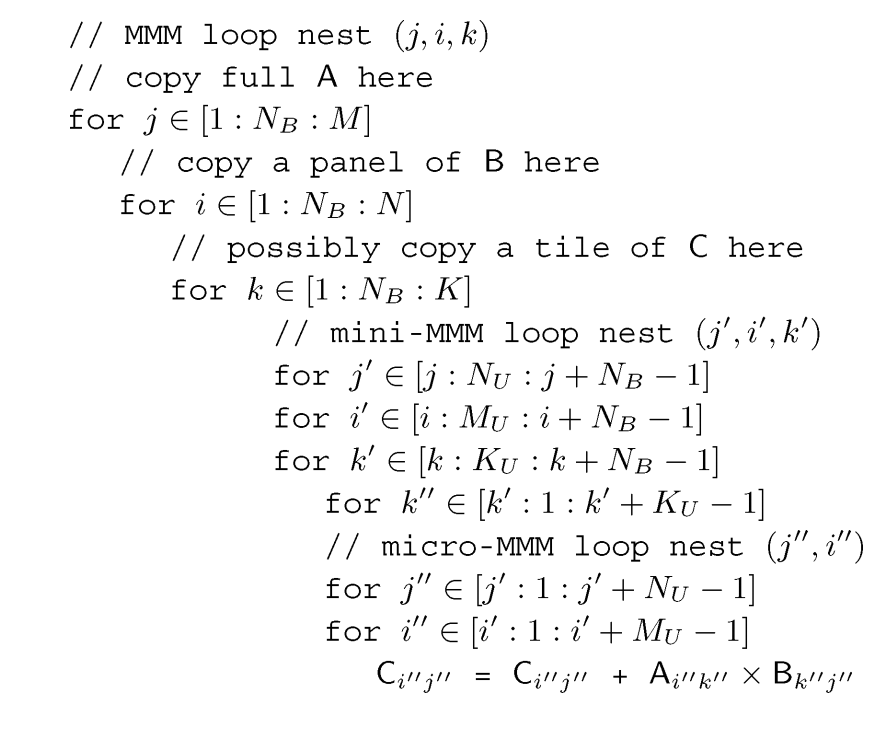
\includegraphics[width=0.9\textwidth]{images/ATLAS_code.png}
    \caption{}
    \label{fig:ATLAS_code}
  \end{subfigure}
  \begin{subfigure}[t]{1.0\linewidth}
    \centering
    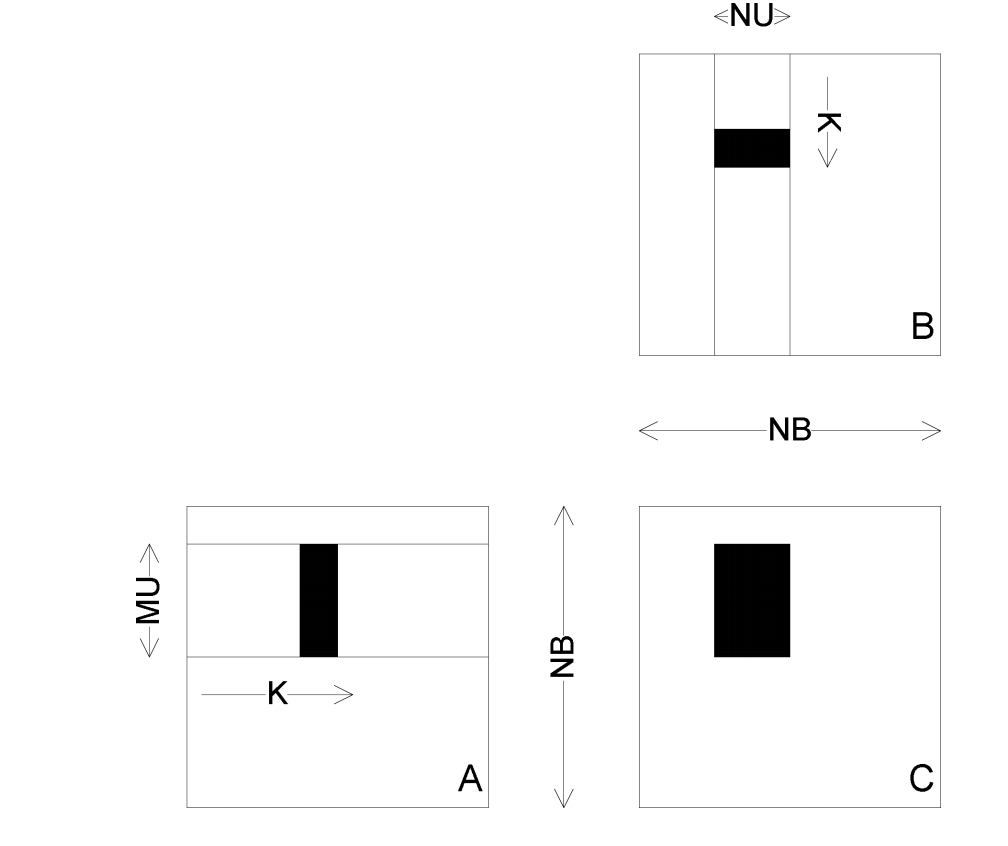
\includegraphics[width=0.9\textwidth]{images/ATLAS_pic.png}
    \caption{}
    \label{fig:ATLAS_pic}
  \end{subfigure}
  \caption{Matrix multiplication tiled for L1 data cache and registers}
  \label{fig:ATLAS}
\end{figure}

  Figure \ref{fig:ATLAS} (adopted from \cite{yotov2005search}) shows the kernel code and pictorial view of matrix multiplication
  blocking for L1 cache and registers. The kernel computes matrix product $C=A*B$. ATLAS first decides the size of the mini-kernel, which is determined
  by knob $NB$, by tiling all three matrices
  to three $NB*NB$ square matrices, as shown in Figure \ref{fig:ATLAS_pic}. Then it optimizes the dimensions of the microkernel based on registers by further dividing them into an $MU*1$ submatrix of $A$ and a $1*NU$ submatrix of $B$. The microkernel accumulates the result into a submatrix with size $MU*NU$ in $C$.
  Furthermore, it is profitable to unroll the microkernel by a factor of $KU$.
  In the above three steps, four optimization parameters $NB$, $MU$, $NU$ and $KU$ have significant impact on performance. \par

  ATLAS also searches the optimal values of other parameters like $LS$, the latency for computation scheduling, $FMA$, if the fused multiply-add unit is available, $IF$, $FF$, $NF$, three fetching parameters
  for load scheduling. For now, we only consider the tiling and unrolling parameters \textbf{\textit{NB}}, \textbf{\textit{MU}}, \textbf{\textit{NU}} and \textbf{\textit{KU}} because 1) the exhaustive search space of them
  is already very huge which typically takes us more than days to generate training data, and 2) the model built from these four parameters are already able to
  generate high performance code and 3) the performance is much less sensitive to the latency and scheduling parameters.
  \par

  ATLAS's empirical technique adopts orthogonal line search to auto-tune its optimization parameters.
  It assumes that the parameters are independent and their optimal values are not relevant to each other. The optimal values can be
  restricted by some architecture features like number of registers, size of L1 cache.\par
  More specifically, it first searches $(MU, NU)$ pairs which meets the register requirement
  \[ MU*NU + MU + NU + LS < NR \]
  where NR is the number of floating point registers.\par
  Then it searches NB, which is the multiple of four in the range of
  \[ [max(20, \sqrt{\frac{C}{3}}), min(80, \sqrt{C}) ] \]
  where C is the size of L1 cache.
  \par
  Finally, it searches KU in the set of
  \[ \{1, 2, 4, 6, 8, 12, 16, 20, 24, 28, 32, \frac{NB}{2}, NB \} \]

  Even though ATLAS empirical can generate good parameters, its search space is still not guaranteed to contain
  the optimal point, and there are still many low performance points in the search space which is unnecessary
  to search. To give the reader a general sense of the result of ATLAS search, on a typical platform with Intel Xeon
  CPU E5-2630 2.3GHz, which has 16 floating point registers and 32kb L1 cache, it takes ATLAS 118s to search 34 data
  points in the $NB\times MU \times NU \times KU$ space and the MFLOPS performance of generated program is 94\% of the
  best of exhaustive search in the same space.


  \subsection{Capri approximate program}
  \label{sec:Capri_intro}
  Capri is a approximate program that helps trade off energy or time with error
  or performance for input programs. Capri focuses on a class of approximate
  programs that we call tunable approximate programs. Intuitively, these
  programs have one or more knobs that can be changed to vary the fidelity of
  produced output. These knobs might control the number of iterations performed
  by a loop \cite{bottou2010large, rinard2007using}, determine the precision with which floating-point
  computations are performed \cite{rubio2013precimonious, schkufza2014stochastic}, and so on.

  There is now a fairly large literature on this subject. Most of these work
  address the solution for \emph{forward problems}: they show that for some
  programs, particular techniques or heuristics can be applied to degrade
  output quality in an acceptable way while reducing energy or running time.
  Another category of approximate problem is called \emph{
  inverse problems}: given some constraint on output quality, how shall we set
  the knobs in order to meet the output quality while reducing the cost (running
  time or error) as much as possible. What makes an approximate problem
  particularly difficult is that for most applications, optimal values of
  knob settings are very dependent on values of inputs. Capri is capable of
  doing both of them as well as the variant introduced by inputs.

  The work flow for Capri can be divided into two phases: training
  phase and testing phase. The training phase is conducted
  offline. Basically, Capri requires the target approximate problem to run
  extensively across the knob space for some inputs and collect cost(running
  time, energy) and error (output quality or performance degradation). A set of
  knob-cost and knob-error pairs are formed for each input. For each input, some
  features are extracted in order to represent the input. These sets of
  knob-cost and knob-error pairs with their input features are fed into
  machine learning boxes in order to build a cost model and a error model
  respectively based on input features and different knob settings.

  During the test phase, Capri would take a
  constraint and an input for the target program as inputs, such as ``a knob
  settings which is 90\% as good as the best rendering quality'', the
  controller would consult the error model and find out
  all the knob settings that is predicted as at least 90\% as good as the best
  one, denoted as feasible region of knobs. Then, the Capri consults the
  cost model for each knob in the feasible region and output the knob setting
  with the least cost. This knob setting with be used for this specific input
  that is predicted to produce a 90\% good result with the least cost.

  The offline training phase is heavy but the online testing phase is really
  light, which usually take few seconds to finish.
  In this project, it would be very intuitive to apply Capri into \atl
  searching process. Capri is able to build the model for \gem performance
  based on knobs in the code on
  different platforms. \atl would take the advantage of this model to prune
  the optimization exploration space and produce an ``enough good'' \gem
  installation. The detailed design choices are explained in
  section~\ref{sec:design}


  %Auto-tuning is a generally used optimization process, which is also
  %approximateable. Intuitively, instead of replacing auto-tuning completely,
  %the process of auto-tunning can be shortened by pruning the search space.
